\chapter{Implementation}
\lstset{language=NoBeardAsm}
\section{Used Technologies}
\subsection{IntelliJ IDEA} 
The implementation of the project is written in Java using the integrated development environment IntelliJ IDEA which is mainly for developing Java based software. Nevertheless, it supports other programming languages too like Scala, Groovy, Kotlin etc\ldots It also support PHP, HTML, CSS3, JavaScript and TypeScript that could be very practicable for web development with the combination of different frameworks like AngularJs, Node.js, SQL Server etc… Another big advantage that IntelliJ IDEA has is the mobile development in Android or Cordova. 
This IDE support a huge variety of benefits such as:
\begin{itemize}
\item Different build systems (maven, gradle, ant, grunt, bower, etc \ldots)
\item Version control systems (Git, Mercurial, Perforce, and SVN)
\item Plugin ecosystem
\item Test runner and coverage
\end{itemize}
More about this topic can be found on this site: \cite{intellij_intellij_nodate}

\subsection{Maven} 
This is a software management and build automation tool which is based on the concept of a project object model (POM). POM is fundamental unit of work in Maven. It is an XML file that resides in the base directory of the project as pom.xml.
The POM contains information about the project and various configuration detail used by Maven to build the project(s).
POM also contains the goals and plugins. While executing a task or goal, Maven looks for the POM in the current directory. It reads the POM, gets the needed configuration information, and then executes the goal. 

One of the biggest features in Maven is the dependency management. Maven automatically downloads the libraries and plug-ins declared in the POM file from the Maven central repository and stores them locally. In simple, when a developer builds a Maven project, all dependency files will be stored in a Maven local repository. So if Maven finds dependency libraries in the Maven local repository, it do not need to download them from the default online Maven central repository multiple time.

By default, the local Maven repository is the .m2 folder
\begin{itemize}
\item \textbf{Unix/Mac OS X: }\lstinline$~/.m2$
\item \textbf{Windows: }\lstinline$C:\Users\{your-username}\.m2$
\end{itemize}

The Maven command \lstinline$mvn install$ builds a project and places its binaries in the local repository. Then other projects can utilize this project by specifying its coordinates in their POMs. Further information about Maven can be found on the official website: \cite{maven_maven_nodate}

\subsection{JavaFX}
JavaFX is a framework which enables developers to design rich client applications that is able to run constantly on different platforms. It offers a wide range of APIs for web rendering, user interface styling and media streaming. JavaFX relies in particular on a scene graph, which manages the individual components of a GUI. It also provides a declarative description of XML-based graphical interfaces with FXML.

The newest JavaFX releases are fully integrated with the current Java SE Runtime Environment(JRE) and Java Development Kit(JDK), which is available for all main desktop platforms. 
More about this topic can be found on the following website: \cite{javafx_main_nodate}

\subsection{Scene Builder} \label{sec:SceneBuilder}
JavaFX Scene Builder is a visual layout tool that generates FXML, an XML-based markup language that lets developers quickly design user interfaces, without any coding. Users just have to drag and drop UI components to the work area. By selecting components users can easily modify their properties or apply style sheets. The XML code for the layout is generated automatically in the background by the tool.

The resulting FXML file can be combined with a Java project by binding the UI to the application’s logic. Every item of the layout view can be assigned with an fx:id to give the controller an easy access of components by the ``@FXML'' annotation. SceneBuilder is an external tool so it has to be downloaded from the official Oracle website and has to be integrated to a Java supporting IDE. 
More about this topic can be found on its website: \cite{scenebuilder_javafx_nodate}

\section{Supporting NoBeard Packages}
The NoBeard Machine is part of the existing NoBeard project. This project already consists of the following packages:
\begin{itemize}
\item \textbf{asm: }NoBeard Assembler to assemble .na files 
\item \textbf{compiler: }NoBeard Compiler to compile .nb source code files
\item \textbf{config: }Hold information of the NoBeard project
\item \textbf{error: }To handle errors that are occurring during compilation or assembly   
\item \textbf{io: }Responsible for reading source files and handling binary files 
\item \textbf{machine: }Implements a virtual machine with components like DataMemory, ProgramMemory, Instructions, etc...  
\item \textbf{scanner: }A scanner converts an input string (generally a whole file) into a list of tokens. These tokens represent things like identifiers, parentheses, operators, etc\ldots
\item \textbf{parser: }It is a program unit that analyses whether a token sequence to a program source text adheres to predetermined grammar rules. If this is not the case, an error message is generated. Otherwise, a structured representation of the program source text is generated that reflects the syntactic structure required by the grammar rules.
\item \textbf{symbolTable: }It is an abstract data type that contains variable names, constants, etc\ldots  
Identifiers are added to the symbol table when they are initially declared. Later, when referring to an identifier, the symbol table is consulted to ensure that the identifier is known and used correctly.
\end{itemize}
However, the most important package for our work is \lstinline$machine$. It defines the interface which the project described here is built upon.
\section{Architecture of the User Interface}
This is the model view controller pattern. The model is responsible for holding data. In our case this is not in a data base but the data is held in the virtual machine. The Model-View-Controller pattern does not require necessarily a database.

The GUI project is build up of three main components as shown in figure~\ref{fig:partsOfGui}. The Controller and the Virtual Machine both of them are running on different threads and are accordingly synchronized. This will be described in detail in section~\ref{sec:synchronization}. The relationship between the controller and view is for event actions and updating of view-components like data memory, output or program flow. The View allows users to call functions from the Controller by clicking on control buttons or by entering inputs. 
\begin{figure}[h] 
	\centering
	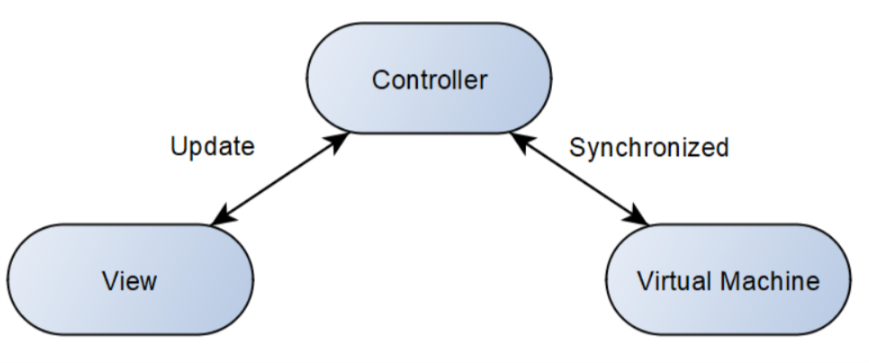
\includegraphics[scale=.70]{images/modelOfGui.png}
	\caption{Main parts of the GUI implementation}
	\label{fig:partsOfGui}
\end{figure}
\subsection{The View}\label{sec:TreeView}
The view is basically a single \lstinline$.fxml$ file which holds the view components of the layout. As figure~\ref{fig:view} shows it was created with an external tool called Scene Builder which is already described in section~\ref{sec:SceneBuilder}.

Each window is made up of an \lstinline$AnchorPane$ \cite{anchorpane_anchorpane_nodate} and is separated by \lstinline$SplitPanes$. An \lstinline$AnchorPane$ enables developers to build flexible user interfaces which can adapt automatically to different screen sizes and orientations. It provides the possibility to constrain the position and size of each element to its parent or siblings. So it becomes very comfortable and easy to size every window as the user wants. Very similar concepts are available in other UI frameworks as Android (\lstinline$LinearLayout$ \cite{android_linearlayout_nodate}) or iOS (\lstinline$UIStackView$ \cite{apple_uistackview_nodate}).

Then each of these \lstinline$AnchorPane$s holds the needed view-components like \lstinline$Button$, \lstinline$TextArea$, \lstinline$TextField$, \lstinline$ListView$ or \lstinline$ScrollPane$.

There are two types of designing and both of them is used in this project to develop a UI that meets all usability requirements.

\subsubsection{Static Design}
Static designing means that all view components are defined in the layout file and not in the Java code. With this type of designing it is pretty easy to build quickly a basic user interface. The developer has only to define the components in an fxml file or place them onto the view via drag and drop with the help of Scene Builder. This part of a project is mostly done by a designer because it does not require a lot of programming knowledge. Listing~\ref{listing:XmlCode} shows a simplified version of how the control buttons were defined in the fxml file.
\lstset{language=XML,style=MyStyle}
\begin{lstlisting}[caption={FXML example}, label=listing:XmlCode]
<AnchorPane>
	<Button fx:id="openButton" onAction="#openFile" text="Open File"/>
	<Button fx:id="startButton" onAction="#startProgram" text="Run"/>
	<Button fx:id="stepButton" onAction="#step" text="Step"/>
	<Button fx:id="continueButton" onAction="#continueToBreakpoint" text="Continue"/>
	<Button fx:id="stopButton" onAction="#stopProgram" text="Stop"/>
</AnchorPane>
\end{lstlisting}

\subsubsection{Dynamic Design}
In dynamic design the already existing view-components is being changed according to run time conditions or to user interactions. This means that the content of statically placed controls changes e.g., by filling or updating a table view. Another typically dynamic designing is when the appearance of these items gets altered through enabling a button or changing its text. This is usually when a user or system triggers an event that matches a particular condition. In this case, the design code has to be mixed with the Java code and therefore programming skills from both sides are necessary. 

Code snippet~\ref{listing:ProgramDataView} shows the \lstinline$fillProgramDataView$ function which is called after a user opens a binary file. This function fills the program window with the content and additionally inserts a \lstinline$CheckBox$ to each line for maintaining the breakpoints.

\lstset{
  language=Java,
  identifierstyle=\color{black},
  keywordstyle=\color{blue},       % keyword style
  stringstyle=\color{forestgreen},     % string literal style
}
  
\begin{lstlisting}[caption={Implementation of program data view},label=listing:ProgramDataView]
private void fillProgramDataView(List<String> programDataList) {
    VBox programData = new VBox();
    for (String lineStr : programDataList)
        addLineToProgramDataView(programData, lineStr);
    programDataView.setContent(programData);
}

private void addLineToProgramDataView(VBox programData, String lineContent) {
    CheckBox line = new CheckBox(lineContent);
    line.setPadding(new Insets(1));
    line.setOnAction((event) -> setClickEventToLine((CheckBox) event.getSource()));
    programData.getChildren().add(line);
    programDataMap.put(getAddressOfProgramLine(line.getText()), line);
}

private void setClickEventToLine(CheckBox breakpoint) {
    if (breakpoint.isSelected())
        machine.addBreakpoint(getAddressOfProgramLine(breakpoint.getText()));
    else
        machine.removeBreakpoint(getAddressOfProgramLine(breakpoint.getText()));
}
\end{lstlisting}

\begin{figure}[h] 
	\centering
	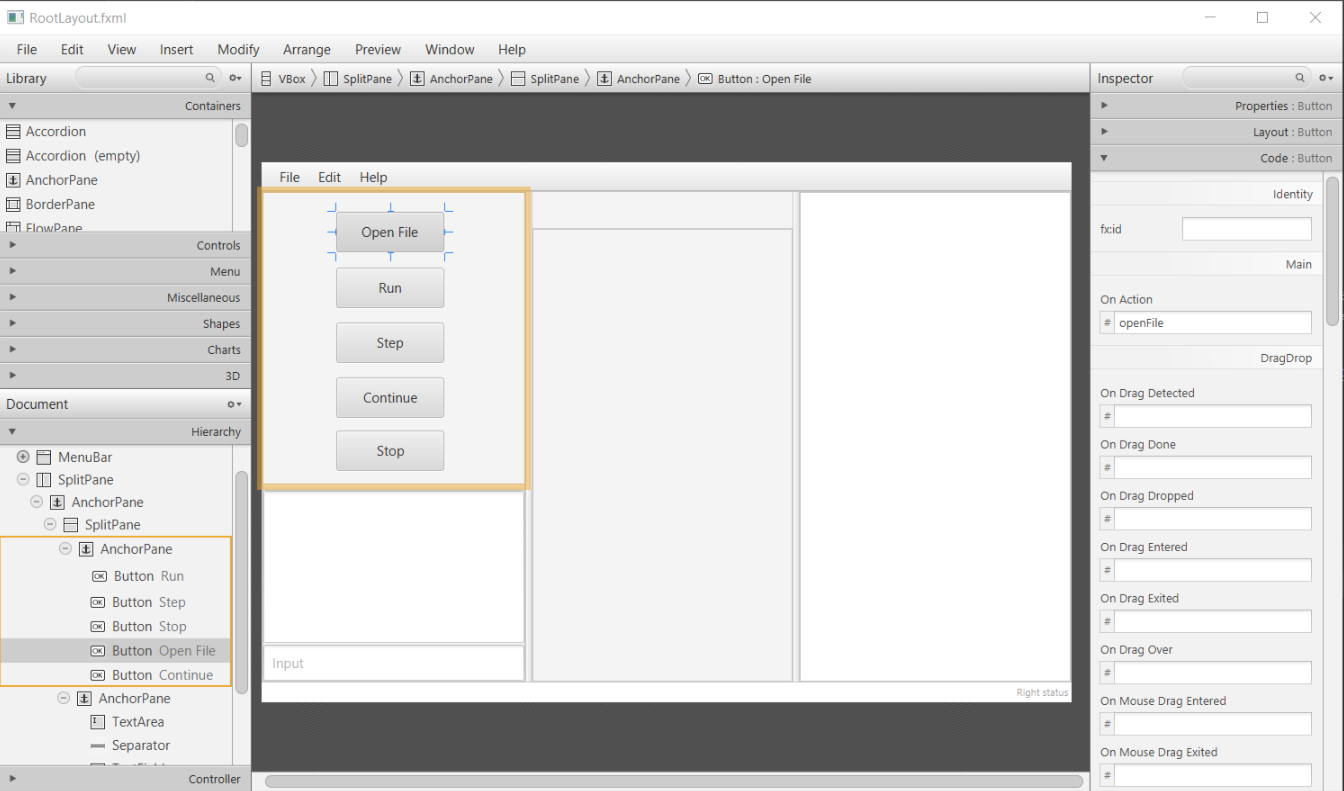
\includegraphics[scale=.55]{images/view.png}
	\caption{Development of the view with Scene Builder}
	\label{fig:view}
\end{figure}
\subsection{The Controller}
The controller is primarily responsible for the coordination and operation of the view and its components. As already described in section~\ref{sec:SceneBuilder} the controller gets access to the view components via the binding of an fx id. To enable this access the view and the controller have to be connected by setting the \lstinline$fx:controller$ attribute of the root view element to the currently used controller. The user interface defined by an FXML file and its controller is loaded into memory by an \lstinline$FXMLLoader$. When the \lstinline$load()$ method is called on the \lstinline$FXMLLoader$, it:
\begin{enumerate}
\item Loads the FXML file
\item Creates an instance of the controller class specified by the \lstinline$fx:controller$ attribute, by calling its no-argument constructor
\item Sets the value of any @FXML-annotated fields in the controller to the elements defined with matching fx:id attributes
\item Registers any event handlers mapping to methods in the controller
\item Calls the \lstinline$initialize()$ method on the controller, if there is one.
\end{enumerate}

Through this advantage event actions like mouse clicks or key presses can be bound between the controller and the view. This could be achieved by setting a name for the ``On Action'' property in Scene Builder and then creating the related function in the controller. The function has to be declared with an \lstinline$@FXML$ annotation and the same name as it was set on the action property of the item.

These action methods accept a single argument of type \lstinline$ActionEvent$. This can be used to get some further information of the fired event like which mouse button was pressed.

Those events have a defined order. The constructor is called before the \lstinline$@FXML$-annotated fields are injected, but the \lstinline$initialize()$ method is called after. This means we can access (and configure) \lstinline$@FXML$-annotated fields in the \lstinline$initialize()$ method, but not in the constructor. It is quite common (at least in simple applications) not to define any constructor in the controller classes.

The other task the controller has to handle is to update the model, i.e., in our case to change the state of the NoBeard machine according to the user commands. So it acts like a bridge to the machine and calls functions like \lstinline$runProgram(int startPc)$, \lstinline$step()$, \lstinline$getCallStack()$ etc\ldots

To achieve this connection between the two components, the controller gets an instance of the NoBeard machine which is being target for NoBeard assembler programs. This happens directly in the \lstinline$initialize()$ method. As said before this method is called automatically and as first when the FX application starts. So every stuff that is needed for the initialization e.g., enabling or disabling controls on the view, is done in this \lstinline$initialize()$ method.

Since the initialization, all other methods can only be invoked by triggering an event like clicking on the ``openFile'' button. However, these event methods gets called under certain conditions that depend on the user. For example, the user has to stop a running program before opening another NoBeard object file. This conclusion gives the controller a defined cycle that the user can execute:
\begin{enumerate}
\item Open file
\item Disassemble file
\item Update view
\item Start program
\end{enumerate}

The opening of a NoBeard object file is operated with the help of a BinaryFileHandler. After an object file is successfully read and program data is available as a binary byte stream it has to be disassembled i.e., that it has to be converted from its binary form to a human readable assembler form.

After this translation is finished the machine has to load the string constants and the program data from the object file into the corresponding memory. Program data is filled in a VBox where each line consists of a CheckBox and an Assembler statement. All of the CheckBoxes get an OnAction event which toggles breakpoints of the machine. This is already demonstrated with the listing~\ref{listing:ProgramDataView}.

When a program is started, a new external thread must be started in which the machine is running separately from the UI. The code~\ref{listing:startingThread} illustrates how the machine gets started on a background thread using a lambda expression.
\begin{lstlisting}[caption={Starting the machine on a new thread},label=listing:startingThread]
@FXML
void startProgram(ActionEvent event) {
    prepareGuiForProgramStart();
    new Thread(() -> {
        machine.runProgram(0);        
    	Platform.runLater(() -> {
            highlightNextInstructionToBeExecuted();
            DataMemoryView.update(this, getRawDataMemoryList());
    }).start();
}
\end{lstlisting}
The reason why and how they run on different threads will be explained in section~\ref{sec:synchronization}. The machine executes step by step every instruction of the program until any interruption. It can be interrupted by a breakpoint, input request or by a \lstinline$halt$ instruction. 

\lstinline$Platform.runLater(java.lang.Runnable runnable)$ is usually used for updating the GUI from a background thread. Java supports \lstinline$Task$ which is a similar concept and can be utilized for the same purpose. 

The method \lstinline$highlightNextInstructionToBeExecuted()$ at line~7 signs the instruction which hast to be executed as next, e.g., if the user press the ``Step'' button then the highlighted assembler statement will be executed. In other words, it shows where the current program counter is.

The final statement in this code snippet is at line~8 which updates the data memory on the view after an interruption, but this will be described in section~\ref{sec:implementationOfDataVisualisation}.

\section{Synchronization of NoBeard Machine and GUI}
\label{sec:synchronization} 
As already mentioned, the NoBeard virtual machine has to run on a background thread. The main reason for this is that there are two different processes using common processing resources. For instance, if they run on the same thread then the user would not be able to make any interactions because the virtual machine locks the main thread. But, even when the virtual machine gets an extra thread there would be still a deadlock because the background thread has to synchronize with the UI thread. So e.g., every time the user has to operate an input, a switch to the UI thread is needed. Otherwise it would cause a critical section between the threads. 

The synchronization of these two threads is implemented with the semaphore construction. A semaphore has a pretty simple usage to solve critical section problems and to achieve process synchronization in the multi processing environment. It is a variable that acts like a traffic light with its \lstinline$acquire()$ and \lstinline$release()$ functions.

The NoBeard Machine contains two interfaces to optimize outputs and inputs on the used device. As soon as the machine executes an input instruction \lstinline$in$, it calls firstly a function from the input interface either \lstinline$hasNextInt()$ or \lstinline$hasNext()$. Both do the same thing, checks whether there is an input by the user or not. The only different is that the one of them also checks if the string is numeric. These functions are overridden in the \lstinline$FxInputDevice$ class where also an instance of the controller is loaded by the constructor. So, by calling one of these \lstinline$hasNext$ function the machine thread should be paused as shown in the code snippet~\ref{listing:Synchronisation1}. To avoid the deadlock, the semaphore from the controller is acquired at this position i.e., at line~11.
\begin{lstlisting}[caption={Synchronisation with semaphore (Part 1)},label=listing:Synchronisation1]
@Override
public boolean hasNextInt() {
    waitForInput();
    return controller.getInput().chars().allMatch( Character::isDigit );
}

private void waitForInput() {
    try {
        Platform.runLater(() -> controller.enableInputView(true));
        controller.getSemaphore().acquire();
    } catch (InterruptedException e) {
        e.printStackTrace();
    }
}
\end{lstlisting}
Now the user can make an input on the UI thread and submit it. To get back to the machine thread, the semaphore hast to be released after the user fires the submit event by pressing the ENTER key. This is demonstrated with the code fragment~\ref{listing:Synchronisation2} more precisely at line~12. Then the machine continues at the same position where the semaphore was acquired, at one of the has Next function and can analyse the provided input string.
\begin{lstlisting}[caption={Synchronisation with semaphore (Part 2)},label=listing:Synchronisation2]
private void makeInputViewReactOnReturn() {
    inputView.setOnKeyPressed(event -> {
        if (event.getCode() == KeyCode.ENTER && inputView != null && 
        		!inputView.getText().isEmpty())
            inputIsAvailable(inputView.getText());
    });
}

private void inputIsAvailable(String providedInput) {
    getOutputView().appendText(providedInput + "\n");
    input = providedInput;
    inputView.clear();
    enableInputView(false);
    getSemaphore().release();
}
\end{lstlisting}
\section{Handling of Breakpoints}
Machine internal handling of breakpoints is done as described in \cite{bendersky_how_nodate}. The implementation for the maintaining of breakpoints is coded with a simple observer pattern design to keep the best performance of the virtual machine. 

The idea of this solution is pretty easy to understand. The machine runs only as long as it is in a \lstinline$running$ state. So, a new instruction is introduced, called \lstinline$break$ which sets the machine into a \lstinline$blocked$ state. This means at the same time that as soon as a user sets a breakpoint on a specified instruction, a change from the original to a \lstinline$break$ instruction is necessary.

The \lstinline$ControlUnit$ which is responsible for execution cycles in the virtual machine is going to be an observable class. Then a new Observer class is implemented which is called \lstinline$BreakpointsHandler$ that is holding all breakpoints in a \lstinline$HashMap$.

\lstinline$private HashMap<Integer, Byte> breakpoints;$
 
This \lstinline$HashMap$ stores the address and the instruction of a selected breakpoint. The \lstinline$BreakpointsHandler$ class contains in all four major functions as shown in the code snippet~\ref{listing:debugger}. Adding and removing breakpoints to or from the \lstinline$HashMap$ and replacing an instruction at a specified address from the program memory to a new one. The selection of a breakpoint on the UI calls the set or remove function from the debugger, as the case may be. As soon as a breakpoint is selected, it will be stored to the \lstinline$HashMap$ with its original instruction and at same time replaces the original instruction by the newly added \lstinline$break$ instruction.
\begin{lstlisting}[caption={Implementation of the debugger},label=listing:debugger]
void setBreakpoint(int atAddress) {
    byte originalInstruction = programMemory.loadByte(atAddress);
    if (originalInstruction != -1) {
        breakpoints.put(atAddress, programMemory.loadByte(atAddress));
        programMemory.replaceInstruction(atAddress, InstructionSet.Instruction.BREAK.getId());
    }
}

void removeBreakpoint(int atAddress) {
    if (breakpoints.containsKey(atAddress)) {
        programMemory.replaceInstruction(atAddress, breakpoints.get(atAddress));
        breakpoints.remove(atAddress);
    } else {
        // force program address error
        programMemory.loadByte(-1);
    }
}

void onStopAtBreakpoint(int atAddress) {
    if (breakpoints.containsKey(atAddress)) {
        programMemory.replaceInstruction(atAddress, breakpoints.get(atAddress));
        programCurrentlyStoppedAtAddress = atAddress;
    }
}

void onContinueFromBreakpoint() {
    programMemory.replaceInstruction(programCurrentlyStoppedAtAddress,
    		InstructionSet.Instruction.BREAK.getId());
}
\end{lstlisting}
This \lstinline$break$ instruction sets the machine to a \lstinline$blocked$ state and notify the observer to change the \lstinline$break$ instruction back to the original one by calling the \lstinline$onStopAtBreakpoint(int atAddress)$ method. 

Now the machine is blocked at a specified breakpoint and the user can take a look to the current memory state and go one step further in the program flow or continue the execution cycle to a next breakpoint. However, when the user wants to step further to execute the current instruction where the breakpoint is, of course again a switch back to the break instruction is needed after the original instruction completed. This is will be done by calling the \lstinline$onContinueFromBreakpoint()$ method.
\section{Visualisation of DataMemory}
\label{sec:implementationOfDataVisualisation}
The visualisation of the data memory gives an overview about string constants and stack frames. As figure~\ref{fig:dataMemoryView} shows the view lists four byte of data on each row starting with the belonging address. 

Logically, the list has to be updated after any interruption by a breakpoint. This is demonstrated with the code snippet~\ref{listing:startingThread}, more precisely at line~7.

\begin{figure}[h] 
	\centering
	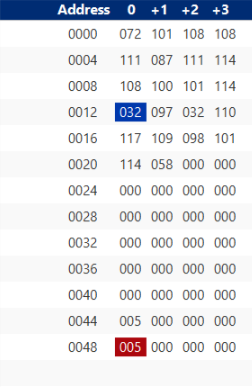
\includegraphics[scale=.99]{images/dataMemory.png}
	\caption{Visualisation of data memory}
	\label{fig:dataMemoryView}
\end{figure}

For the visualisation of these data a \lstinline$ListView$ is defined on the view which is one of the best choice for this purpose. 
The updating of data memory view has defined a cycle. Firstly a function iterates through the memory until the current stack pointer and groups all data into four bytes and finally stores them into an observable collection of strings. Then this collection is assigned to \lstinline$ListView$ items that are visible on the view. Each row of the \lstinline$ListView$ contains now a line of string filled with the address and four pure data. 

Since each item in a \lstinline$ListView$ is represented by an instance of the \lstinline$ListCell$ class, a row can be customized to get a nice structure like in figure~\ref{fig:dataMemoryView}. This customisation of a cell can be achieved with the \lstinline$cellFactory$ API. The cell factory is called by the platform whenever it determines that a new cell needs to be created. 
To specialize the \lstinline$Cell$ used for the \lstinline$ListView$, an implementation of the \lstinline$cellFactory$ callback function has to be provided.
\begin{lstlisting}[caption={Implementation of the data memory view using cell factory},label=listing:CellFactory]
static void update(Controller controller, ObservableList<String> content) {
    controller.getDataMemoryListView().setItems(content);
    controller.getDataMemoryListView().setCellFactory(list -> new ListCell<String>() {
        int framePointer = controller.getMachine().getCallStack().getFramePointer();
        int stackPointer = controller.getMachine().getCallStack().getStackPointer();
        static final int INDEX_OF_ADDRESS = 0;

        @Override
        protected void updateItem(String item, boolean empty) {
            super.updateItem(item, empty);
            if (item != null) {
                createDataLine(item);
            }
        }

        private void createDataLine(String item) {
            HBox line = new HBox();
            int firstAddressInLine = getIndex() * 4;
            convertStringToLabels(firstAddressInLine, item).forEach(line.getChildren()::add);
            setContextMenuToDataCells(line);
            setGraphic(line);
        }

        private List<Label> convertStringToLabels(int firstAddressInLine, String line) {
            String[] lineContent = splitDataLine(line);
            List<Label> result = createLabelForAddress(lineContent[INDEX_OF_ADDRESS]);
            int currentAddress = firstAddressInLine;
            for (int i = 1; i < lineContent.length; i++) {
                if (currentAddress == framePointer)
                    result.add(createHighlightedLabel(lineContent[i], "#0038AC"));
                else if (currentAddress == stackPointer)
                    result.add(createHighlightedLabel(lineContent[i], "#AC080E"));
                else
                    result.add(createNormalLabel(lineContent[i]));
                currentAddress++;
            }
            return result;
        }
        ...
\end{lstlisting}

In the code example~\ref{listing:CellFactory} an anonymous inner class is created using lambda expression, that simply returns instances of \lstinline$ListCell$ overriding the \lstinline$updateItem$ method. This method is called whenever the item in the cell changes, for example when the user scrolls the \lstinline$ListView$ or the NoBeard machine updates the data memory (and the cell is reused to represent some different item in the \lstinline$ListView$). Because of this, there is no need to manage bindings - simply reacting to the change in items when this method occurs. In this example, whenever the item changes, we update the cell text property, and also modify the text fill to ensure that we get the correct visuals.
So each row of the list view will be separated in five labels, one for the address and four with one byte data. Labels with a given id can be easily styled in a extra CSS file by setting paddings or backgroundcolor. The data labels get a click event to open up a context menu where the following four functions are available:
\begin{itemize}
\item Convert data to a single character
\item Convert a line of data to four characters
\item Convert a four byte of data to a single integer
\item Convert a translated line of data back to raw data
\end{itemize}
A context menu is a pop-up window that appears in response to a mouse click. The context menu can contain one or more menu items. It is quite similar to a Menu and consists of items with types of \lstinline$MenuItem$, \lstinline$CheckMenuItem$, \lstinline$RadioMenuItem$ or \lstinline$SeparatorMenuItem$. In our case, the context menu holds only items with the default type which is \lstinline$MenuItem$. Each \lstinline$MenuItem$ gets an \lstinline$OnAction$ event where the conversion method is being called. So, when the user clicks on one of these \lstinline$MenuItem$ the translation will be started.
Listing~\ref{listing:ContextMenu} shows how to add a \lstinline$ContextMenu$ to our \lstinline$ListView$ and display it when a user clicks with the right mouse button on an item from the \lstinline$ListView$. 

\begin{lstlisting}[caption={Context menu},label=listing:ContextMenu]
controller.getDataMemoryListView().setContextMenu(contextMenu);
controller.getDataMemoryListView().setOnContextMenuRequested(event -> {
    contextMenu.show(controller.getDataMemoryListView(),
     event.getScreenX(), event.getScreenY());
    event.consume();
});
\end{lstlisting}
With this solution we can only convert entire lines of the \lstinline$DataMemoryView$, since only access to a selected index of a \lstinline$ListView$ is possible. For example, if a user wants to translate a cell into a single char or to view an integer, then the desired address is needed for the conversion. When translating a whole line, we get the address because every line begins with the starting address but when a user click on a random cell, we get only the address of the first byte from the row. 

To solve this problem each \lstinline$Label$ (cell) has to react when a right mouse button is being clicked. With the \lstinline$setOnMouseClicked$ method an event can be assigned to a \lstinline$Label$ where the needed extra \lstinline$MenuItem$s will be added to the \lstinline$ContextMenu$ of the \lstinline$ListView$. Each \lstinline$MenuItem$ get again an \lstinline$OnAction$ event where the translation method will be called but now the needed address or data can passed as an argument. 

For the implementation of these conversation functions a separated \lstinline$DataMemoryConverter$ class is introduced. The conversion of a single byte to character is handled by translating the ASCII value which is the current byte to a char. 

For integers it is a bit more complex because a single integer has to take four byte of data. If all the four bytes are not aligned in one row, the rest bytes has to be occupied from the next row. Then the first cell on the desired address is being changed to the translated integer and the next three cell has to be replaced by empty labels.